\section{Introduktion}
\begin{itemize}
	\item Base station
	\item End systems
	\item Dækning
	\item 802.11 protokollen
\end{itemize}

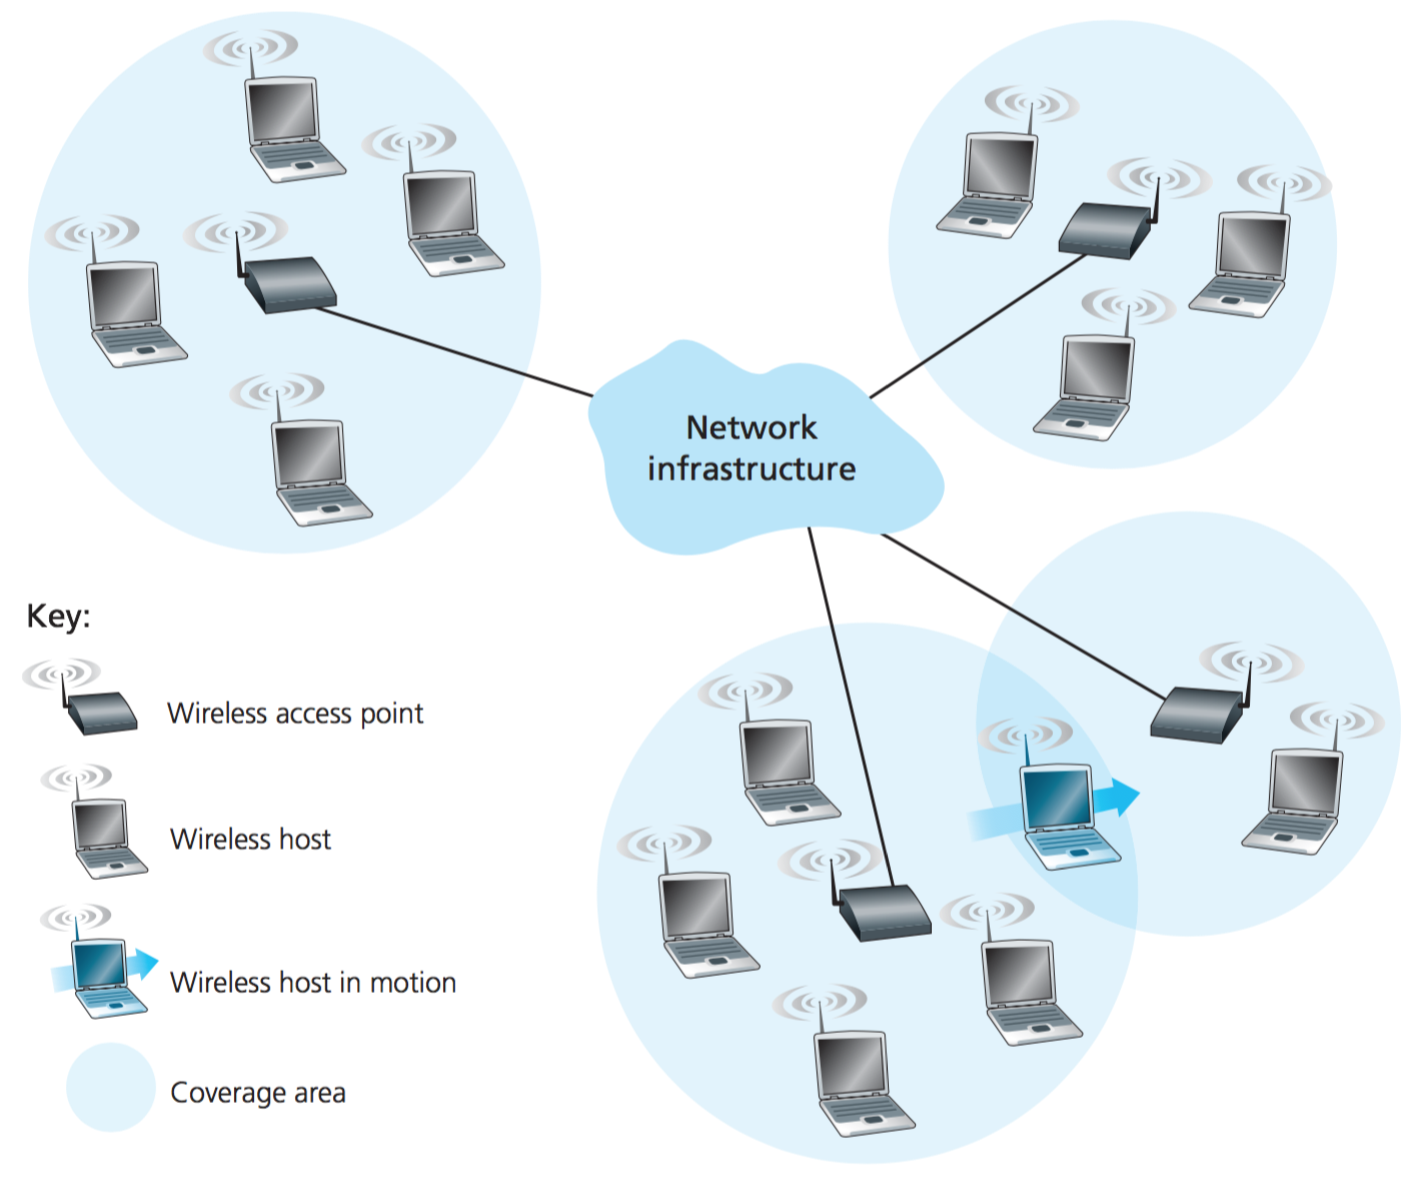
\includegraphics[scale=0.6]{6-wireless/wireless-network.png}

\section{Ulemper ved WiFi}
\begin{itemize}
	\item Svækket styrke hvis signalet skal passere igennem objekter/vægge osv
	\item Forstyrrelser fra andre kilder på samme frekvensbånd (telefoner, mikrobølgeovne)
	\item Multipath propagation: Signal reflekteres 
	\item Disse svagheder resulterer i bit errors
\end{itemize}

\section{Bit Errors}
\begin{itemize}
	\item SNR = Signal-to-Noise Ratio, måles i dB
	\item BER = Bit Error Rate
	\item Højere SNR = lavere BER
\end{itemize}

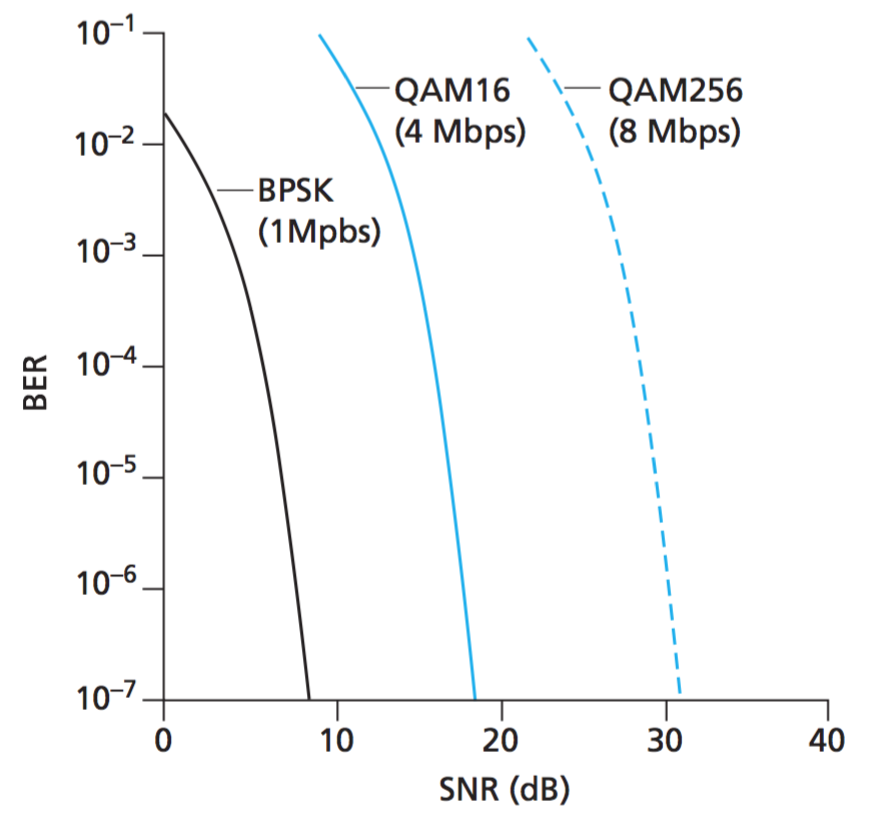
\includegraphics[scale=0.6]{6-wireless/snr-to-ber.png}

\section{Multiple Access}
\begin{itemize}
	\item Channel partitioning protocols - CDMA (Code Division Multiple Access)
	\item Random access protocols - CSMA
	\item Taking-turns protocols
	\item 802.11 bruger CSMA/CA - Collision Avoidance, Ethernet = Collision Detection
\end{itemize}